\documentclass[letterpaper,11pt]{report}

\usepackage{fullpage}
\usepackage{verbatim}
\usepackage{cite}
\usepackage{setspace}
\usepackage{fancyhdr}
\usepackage[small]{caption}
\usepackage{graphics}
\usepackage{color}
\usepackage{hyperref}
\usepackage[dvips]{graphicx}
\usepackage{amsmath}
\usepackage{amssymb}
\usepackage{tikz}
\usetikzlibrary{shapes.geometric, arrows.meta, positioning, calc, fit, backgrounds}
\usepackage{listings}
\usepackage{forest}
\usepackage{booktabs}
\usepackage{multirow}
\usepackage{array}

% Listing style for code
\lstset{
  basicstyle=\ttfamily\footnotesize,
  keywordstyle=\bfseries\color{blue!70!black},
  commentstyle=\itshape\color{green!40!black},
  stringstyle=\color{red!60!black},
  frame=single,
  breaklines=true,
  numbers=left,
  numberstyle=\tiny\color{gray},
  captionpos=b,
  xleftmargin=1.5em,
  framexleftmargin=1.5em,
}

% Paper conservation layout. Long live the trees!!
\setlength{\oddsidemargin}{-0.4mm} % 25 mm left margin
\setlength{\evensidemargin}{\oddsidemargin}
\setlength{\textwidth}{160mm}      % 25 mm right margin
\setlength{\topmargin}{-5.4mm}     % 20 mm top margin
\setlength{\headheight}{5mm}
\setlength{\headsep}{5mm}
\setlength{\footskip}{10mm}
\setlength{\textheight}{237mm}     % 20 mm bottom margin

\setlength{\parskip}{1ex}
\parindent 0in

\def\title{High Frequency Signal Generation Engine for Cross-Border Arbitrage (Phase 2)}

% Cover Page Definitions
\def\addrone{Your address}
\def\addrtwo{Your city}
\def\degree{B.Tech. in Computer Science and Social Sciences}
\def\btptrack{Entrepreneurship Track}
\def\submissiondate{April 18, 2026}
\def\supervisorone{Mr. Pankaj Vajpayee}

\begin{document}

% --- INLINED COVER PAGE ---
\thispagestyle{empty}
\vspace{5.65in}
\begin{center}
\vspace{5.65in}

{\LARGE \bf { High Frequency Signal Generation Engine for Cross-Border Arbitrage } }  
\vspace{.3in}

{\Large{Prakhar}} \\  
{\large{2022360}} \\  
\vspace{1em}
{\Large{Pooja Nardeo Singh}} \\  
{\large{2022356}} \\  
\vspace{1em}
{\Large{Rishit Gupta}} \\  
{\large{2022406}} \\  
\vspace{.1in} 

\vspace{.65in}
\vspace{.65in}

{BTP report submitted in partial fulfillment of the requirements \\for the Degree of B.Tech.}

on {April, 21 2026} \\
\vspace{.65in}

\textbf{BTP Track}: \btptrack\\
\quad\\

{\textbf{BTP Advisor} \\ 
\supervisorone \\ 
\vspace{3.0in}

{Indraprastha Institute of Information Technology\\
New Delhi}

\end{center}
% --- END COVER PAGE ---

\newpage

\begin{center}
\textbf{\Large Student's Declaration}\label{section:declaration}
\end{center}

I hereby declare that the work presented in the report entitled \textbf{``High Frequency Signal Generation Engine for Cross Border Arbitrage"} submitted by me for the partial fulfillment of the requirements for the degree of \emph{Bachelor of Technology} at Indraprastha Institute of Information Technology, Delhi, is an authentic record of my work carried out under guidance of \textbf{Prof. Pankaj Vajpayee}. Due acknowledgements have been given in the report to all material used. This work has not been submitted anywhere else for the reward of any other degree.
\\ \vspace{0.5in}

\textbf{..............................}\hfill
\textbf{ Place \& Date: Delhi, 21/04/2026} \\
\textbf{Prakhar}\\
\textbf{Pooja Nardeo Singh}\\
\textbf{Rishit Gupta}

\vspace{3in}

\begin{center}
\textbf{\Large Certificate} \label{section:certificate}
\end{center}

This is to certify that the above statement made by the candidate is correct to the best of my knowledge.
\\ \vspace{0.4in}

\textbf{..............................}\hfill
\textbf{ Place \& Date: Delhi, 21/04/2026} \\
\textbf{Prof. Pankaj Vajpayee}\\

\pagebreak

\begin{abstract}
The evolution of algorithmic trading necessitates a fundamental shift from isolated predictive models toward holistic, integrated systems capable of dynamically responding to non-linear market microstructures. This Phase 2 report presents the complete design, implementation, and empirical validation of a probabilistic, risk-aware trading signal generation engine that extends the foundational high-frequency data ingestion and deterministic arbitrage detection system established in Phase 1.

Phase 1 established the core streaming architecture, utilizing Redpanda (a C++-native distributed streaming broker) and QuestDB (a high-performance time-series database) to detect deterministic arbitrage loops via an optimized Shortest Path Faster Algorithm (SPFA) implemented in C++ with PyBind11 bindings. Phase 2 significantly expands this mandate by introducing four major subsystems: (1) a \textbf{Graph Embedding Pipeline} using Node2Vec random walks and KMeans clustering to dynamically identify co-moving currency pair candidates across 26 FX instruments spanning 15 currencies; (2) a \textbf{Statistical Arbitrage Module} that validates pair candidates through Engle-Granger cointegration testing and calibrates the continuous-time Ornstein-Uhlenbeck stochastic differential equation via Maximum Likelihood Estimation to generate z-score-based trading signals; (3) a \textbf{Hybrid Machine Learning Pipeline} that stacks ARIMA(2,0,1)/GARCH(1,1) econometric feature extractors, a Keras LSTM sequence encoder, and an XGBoost binary classifier to produce directional momentum probabilities; and (4) a \textbf{Simulation-Based Risk Layer} that employs Cholesky-decomposed Monte Carlo simulation (10,000 paths) to compute Conditional Value at Risk (CVaR) at the 95\% and 99\% confidence levels, which directly constrains dynamic capital allocation via a Fractional Kelly position sizing model.

The complete system comprises 5 containerized services orchestrated via Docker Compose, processes 26 currency pairs across 15 global currencies, and has been validated through a comprehensive integration test demonstrating all subsystems operating end-to-end.
\\

\vspace{2in}
Keywords: Arbitrage, Graph Algorithms, Streaming Graphs, Redpanda, QuestDB, Node2Vec, Cointegration, Ornstein-Uhlenbeck, LSTM, XGBoost, ARIMA, GARCH, CVaR, Kelly Criterion, Monte Carlo Simulation.
\end{abstract}

\newpage

\section*{Acknowledgments}\label{section:acknowledgments}
\pagestyle{plain}
\pagenumbering{roman}

We would like to express our heartfelt gratitude to Professor Pankaj Vajpayee for his invaluable guidance, encouragement, and support throughout this project. His expertise and insights have been instrumental in shaping the direction of our work and overcoming the challenges faced during its execution. We are also thankful to the open-source communities of Redpanda, QuestDB, and the Python quantitative finance ecosystem for providing the robust tools that form the backbone of this system.
\vspace{2in}

\newpage

\tableofcontents
\newpage

\pagenumbering{arabic}
\setcounter{page}{1}

% ======================================================================
\chapter{Phase 1 Recap: Foundational Architecture}
% ======================================================================

\section{Motivation and Problem Statement}

Modern financial markets approach informational efficiency yet operate across fragmented trading venues, regulatory regimes, and liquidity pools. Under classical asset pricing theory, efficient markets enforce the \textbf{Law of One Price (LOOP)}, which asserts that economically identical assets should trade at the same price when expressed in a common numeraire. Despite this theoretical guarantee, empirical observations consistently report short-lived pricing dislocations induced by communication delays, disparate market microstructures, and exchange-specific fees.

The objective of Phase 1 was to design and implement a hybrid high-frequency system capable of:
\begin{itemize}
    \item Ingesting real-time tick-level foreign exchange (FX) quotes at microsecond resolution.
    \item Maintaining a continuously updated directed \textbf{currency exchange graph}, where nodes denote currencies and edges encode exchange rates.
    \item Detecting profitable arbitrage loops \emph{dynamically} without assuming a fixed cycle depth.
    \item Ensuring minimal and deterministic end-to-end latency using a fully event-driven design.
\end{itemize}

\section{Fundamentals of Arbitrage and Graph Representation}

Arbitrage is a trading strategy that requires no initial net capital investment, entails no exposure to market risk, and yields non-negative profit with strictly positive probability. In FX markets, trades occur over pairs $A/B$, representing the price of one unit of currency $A$ expressed in currency $B$.

To detect arbitrage, we modeled the FX market as a directed weighted graph $G = (V, E)$, where vertices represent currencies and edges represent available exchange pairings. A fee-adjusted arbitrage cycle $\gamma = (c_1, c_2, \dots, c_n, c_1)$ is profitable if the compounded exchange rate exceeds unity:
$$\prod_{i=1}^{n} (1 - f_{c_i,c_{i+1}}) \cdot R_{c_i,c_{i+1}} > 1$$
where $f_{c_i,c_{i+1}}$ denotes the friction (fees) for converting currency $c_i$ to $c_{i+1}$ and $R_{c_i,c_{i+1}}$ is the exchange rate.

Because classical shortest-path algorithms operate on additive weights, we applied a logarithmic transformation to the edge weights:
$$w(u, v) = - \log((1 - f_{uv}) \cdot \text{Rate}_{u,v})$$
With this transformation, negative cycle detection became equivalent to arbitrage identification:
$$\sum_{(u,v) \in \gamma} w(u,v) < 0 \iff \prod_{\gamma} (1 - f_{uv}) \cdot R_{u,v} > 1$$

We utilized the \textbf{Shortest Path Faster Algorithm (SPFA)} due to its event-reactive relaxation behavior and empirical $O(kE)$ complexity on sparse graphs, making it ideal for streaming currency graphs where $|E| \ll |V|^2$.

\section{System Architecture Summary (Phase 1)}

The Phase 1 architecture evolved through rigorous performance evaluation and technology pivots:
\begin{itemize}
    \item \textbf{Streaming Backbone:} We transitioned from Apache Kafka, which suffered from JVM garbage-collection latency spikes, to \textbf{Redpanda}, a C++-native distributed streaming broker that eliminates JVM overhead through a thread-per-core execution model and direct disk I/O.
    \item \textbf{Compute Engine:} To bypass Python's Global Interpreter Lock (GIL), we implemented a \textbf{C++ Compute Core} (401 lines) containing the graph data structure, SPFA implementation, and DFS-based $n$-order cycle detection. This core is exposed to Python via \textbf{PyBind11}, enabling the orchestration layer to leverage Python's mature data-science ecosystem without carrying critical-path compute overhead.
    \item \textbf{Persistence Sink:} We adopted \textbf{QuestDB}, an ultra-fast time-series database supporting Influx Line Protocol (ILP), enabling non-blocking historical data storage via \texttt{SYMBOL} string interning for fast indexed filtering.
\end{itemize}

Phase 1 successfully validated the algorithmic correctness of cycle feasibility detection within millisecond-scale reaction times under synthetic stress testing. However, it was strictly limited to deterministic, instantaneous arbitrage. Phase 2 transitions the project to exploit probabilistic inefficiencies using statistical modeling, machine learning, and stochastic calculus.


% ======================================================================
\chapter{Phase 2 Goals and Scope}
% ======================================================================

Phase 2 shifts the paradigm from simple deterministic graph cycles to predictive, risk-managed statistical arbitrage across a dynamic multi-asset universe. The key objectives are:

\begin{enumerate}
    \item \textbf{Dynamic Pair Selection:} Use graph machine learning (Node2Vec embeddings) to automatically discover structurally similar currency pairs from a live correlation network, replacing static pair selection.
    \item \textbf{Statistical Arbitrage:} Validate candidate pairs through Engle-Granger cointegration testing, then calibrate the Ornstein-Uhlenbeck stochastic process to generate mean-reversion trading signals with quantifiable confidence.
    \item \textbf{Hybrid Predictive Pipeline:} Stack classical econometric baselines (ARIMA, GARCH) with deep learning (LSTM) and gradient-boosted trees (XGBoost) to generate directional momentum probability scores.
    \item \textbf{Risk-Aware Position Sizing:} Implement Monte Carlo simulation with Cholesky-decomposed correlated paths to compute CVaR tail-risk bounds, and use Fractional Kelly Criterion for position sizing constrained by risk limits.
    \item \textbf{End-to-End Integration:} Wire all subsystems into a single orchestrated data pipeline running across 5 containerized services with real-time Kafka-based event propagation.
\end{enumerate}

\section{Expanded Currency Universe}

Phase 2 significantly expands the currency universe from 7 major currencies to \textbf{15 currencies} spanning major, cross, and emerging-market pairs:

\begin{table}[h]
\centering
\caption{Phase 2 Currency Universe — 15 currencies, 26 tradeable pairs}
\begin{tabular}{llll}
\toprule
\textbf{Category} & \textbf{Currency} & \textbf{Code} & \textbf{Example Pairs} \\
\midrule
\multirow{7}{*}{Major} & Euro & EUR & EUR/USD, EUR/JPY \\
 & US Dollar & USD & USD/JPY, USD/CAD \\
 & Japanese Yen & JPY & GBP/JPY, AUD/JPY \\
 & British Pound & GBP & GBP/USD, EUR/GBP \\
 & Australian Dollar & AUD & AUD/USD, AUD/SGD \\
 & Canadian Dollar & CAD & USD/CAD \\
 & Swiss Franc & CHF & USD/CHF, EUR/CHF \\
\midrule
\multirow{8}{*}{Emerging} & Indian Rupee & INR & USD/INR, EUR/INR \\
 & Chinese Yuan & CNY & USD/CNY, EUR/CNY \\
 & Russian Ruble & RUB & USD/RUB \\
 & Kuwaiti Dinar & KWD & USD/KWD \\
 & Singapore Dollar & SGD & USD/SGD, EUR/SGD \\
 & Hong Kong Dollar & HKD & USD/HKD, GBP/HKD \\
 & Brazilian Real & BRL & USD/BRL \\
 & Mexican Peso & MXN & USD/MXN \\
\bottomrule
\end{tabular}
\end{table}

The system models realistic cross-currency relationships using 11 triangular consistency constraints (e.g., EUR/JPY $\approx$ EUR/USD $\times$ USD/JPY) with correlated Geometric Brownian Motion price dynamics and GARCH-like volatility regime switches in the mock data generator.


% ======================================================================
\chapter{Project Structure and Architecture}
% ======================================================================

\section{Repository Layout}

The project is organized into modular Python packages, each responsible for a distinct functional layer of the trading system:

\begin{verbatim}
cross-border-arb/
├── docker-compose.yml        # 5-service Docker orchestration
├── run_system.py             # Master orchestrator (358 lines)
├── requirements.txt          # 16 dependencies across 6 categories
├── test_phase2.py            # Integration test suite (579 lines)
│
├── ingestion/                # Data Ingestion Layer
│   └── main.py               # Realistic mock FX generator (413 lines)
│
├── engine/                   # C++ Arbitrage Engine
│   ├── src/graph.cpp          # SPFA + DFS graph core (401 lines)
│   ├── main.py                # Kafka consumer + signal router
│   ├── setup.py               # PyBind11 build configuration
│   └── visualize_graph.py     # NetworkX graph renderer
│
├── streaming/                # Stream Processing Layer
│   ├── processor.py           # OHLCV aggregation + features (567 lines)
│   └── correlation.py         # Rolling Pearson correlation engine
│
├── strategy/                 # Strategy Engine
│   ├── main.py                # Orchestrator (398 lines)
│   ├── graph_embeddings.py    # Node2Vec + KMeans pipeline
│   ├── cointegration.py       # Engle-Granger testing
│   ├── stat_arb.py            # OU process calibration + signals
│   └── ml/                    # Machine Learning Pipeline
│       ├── pipeline.py        # End-to-end ML orchestrator
│       ├── econometrics.py    # ARIMA(2,0,1) + GARCH(1,1)
│       ├── lstm_model.py      # Keras LSTM feature extractor
│       └── xgboost_classifier.py  # XGBoost direction classifier
│
├── risk/                     # Risk Management Layer
│   ├── monte_carlo.py         # Cholesky MC simulation engine
│   └── position_sizing.py     # Fractional Kelly position sizer
│
├── backtest/                 # Backtesting Framework
│   ├── replay.py              # Historical data replay engine
│   └── metrics.py             # Sharpe, Sortino, Max DD, etc.
│
├── storage/                  # Database Initialization
│   └── main.py                # QuestDB table creation
│
├── scripts/
│   └── init_questdb.py        # QuestDB schema initialization
│
├── utils/
│   └── logger.py              # Centralized logging
│
├── models/                   # Trained Model Artifacts
│   ├── xgboost_direction.json # Serialized XGBoost model
│   └── xgboost_direction_meta.json  # Feature importance metadata
│
└── data/                     # Docker volume mounts
    ├── redpanda/              # Redpanda data directory
    ├── questdb/               # QuestDB data directory
    └── flink/                 # Flink checkpoints
\end{verbatim}

\section{Containerized Infrastructure}

The infrastructure layer is fully containerized using Docker Compose, orchestrating 5 independent services on a shared \texttt{arb-net} bridge network:

\begin{table}[h]
\centering
\caption{Docker Compose Service Configuration}
\begin{tabular}{lllp{5.5cm}}
\toprule
\textbf{Service} & \textbf{Image} & \textbf{Port(s)} & \textbf{Role} \\
\midrule
\texttt{redpanda} & \texttt{redpandadata/redpanda:latest} & 19092, 9644 & C++-native Kafka-compatible streaming broker \\
\texttt{questdb} & \texttt{questdb/questdb:latest} & 9000, 9009, 8812 & Time-series database (REST, ILP, PostgreSQL) \\
\texttt{console} & \texttt{redpandadata/console:latest} & 8080 & Redpanda web UI for topic inspection \\
\texttt{flink-jm} & \texttt{flink:1.18-java11} & 8081 & Flink JobManager (stream processing) \\
\texttt{flink-tm} & \texttt{flink:1.18-java11} & --- & Flink TaskManager (4 task slots) \\
\bottomrule
\end{tabular}
\end{table}

Redpanda is configured with 1 SMP thread and 1\,GB memory allocation, running in overprovisioned mode suitable for development. It exposes both internal (\texttt{:9092}) and external (\texttt{:19092}) Kafka listeners. QuestDB exposes three protocols: REST API on port 9000, Influx Line Protocol (ILP) on port 9009 for high-throughput tick ingestion, and PostgreSQL wire protocol on port 8812 for SQL-based analytical queries.

\section{End-to-End Data Flow Architecture}

The system operates as a multi-stage event-driven pipeline. Each stage consumes from and produces to Kafka topics, ensuring complete decoupling between ingestion, computation, and persistence:

\begin{figure}[h]
\centering
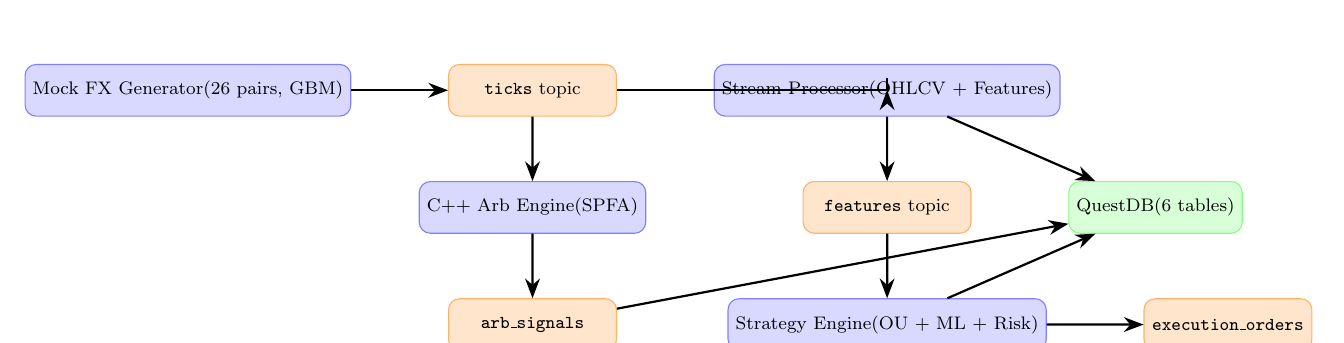
\begin{tikzpicture}[
    scale=0.82, transform shape,
    node distance=1.0cm and 1.5cm,
    box/.style={rectangle, draw, rounded corners, minimum width=2.6cm, minimum height=0.8cm, text centered, font=\footnotesize},
    kafka/.style={box, fill=orange!20, draw=orange!60},
    service/.style={box, fill=blue!15, draw=blue!50},
    db/.style={box, fill=green!15, draw=green!50},
    arrow/.style={-{Stealth[length=2.5mm]}, thick},
]

% Row 1: Ingestion
\node[service] (ingest) {Mock FX Generator\\(26 pairs, GBM)};
\node[kafka, right=of ingest] (ticks) {\texttt{ticks} topic};

% Row 2: Processing
\node[service, below=of ticks] (engine) {C++ Arb Engine\\(SPFA)};
\node[service, right=of ticks] (stream) {Stream Processor\\(OHLCV + Features)};
\node[kafka, below=of stream] (features) {\texttt{features} topic};

% Row 3: Strategy
\node[service, below=of features] (strategy) {Strategy Engine\\(OU + ML + Risk)};
\node[kafka, right=of strategy] (orders) {\texttt{execution\_orders}};

% DB
\node[db, right=of features] (questdb) {QuestDB\\(6 tables)};

% Signal topic
\node[kafka, below=of engine] (signals) {\texttt{arb\_signals}};

% Arrows
\draw[arrow] (ingest) -- (ticks);
\draw[arrow] (ticks) -- (engine);
\draw[arrow] (ticks) -| (stream);
\draw[arrow] (engine) -- (signals);
\draw[arrow] (signals) -- (questdb);
\draw[arrow] (stream) -- (features);
\draw[arrow] (features) -- (strategy);
\draw[arrow] (strategy) -- (orders);
\draw[arrow] (stream) -- (questdb);
\draw[arrow] (strategy) -- (questdb);

\end{tikzpicture}
\caption{Phase 2 End-to-End Data Flow: Ingestion $\to$ Kafka $\to$ Processing $\to$ Strategy $\to$ Execution}
\end{figure}

\section{Kafka Topic Architecture}

The system utilizes four distinct Kafka topics for inter-service communication:

\begin{table}[h]
\centering
\caption{Kafka/Redpanda Topic Configuration}
\begin{tabular}{llp{7cm}}
\toprule
\textbf{Topic} & \textbf{Producer} & \textbf{Content} \\
\midrule
\texttt{ticks} & Ingestion & Raw FX tick data in OANDA v20 JSON format (bid, ask, spread, volume per instrument) \\
\texttt{features} & Stream Processor & Enriched feature vectors (mid, log-return, rolling statistics, spread) per tick \\
\texttt{arbitrage\_signals} & C++ Engine & Detected arbitrage cycles with profit percentage and path \\
\texttt{execution\_orders} & Strategy Engine & Risk-approved trade orders with position sizing \\
\bottomrule
\end{tabular}
\end{table}

\section{QuestDB Schema Design}

QuestDB stores 6 tables using the \texttt{SYMBOL} type for currency pair identifiers, enabling integer-level comparisons via string interning:

\begin{table}[h]
\centering
\caption{QuestDB Table Schema Summary}
\begin{tabular}{llp{6.5cm}}
\toprule
\textbf{Table} & \textbf{Key Columns} & \textbf{Purpose} \\
\midrule
\texttt{market\_ticks} & symbol, bid, ask, mid, spread & Raw tick persistence \\
\texttt{ohlcv\_1m} & symbol, open, high, low, close, vwap & 1-minute OHLCV bars \\
\texttt{model\_features} & symbol, log\_return, rolling stats & Computed ML features \\
\texttt{correlation\_matrix} & symbol\_a, symbol\_b, correlation & Pairwise correlation snapshots \\
\texttt{arbitrage\_signals} & signal\_id, path, profit\_pct & Detected arbitrage opportunities \\
\texttt{risk\_metrics} & symbol, var\_95, cvar\_95, kelly & Risk and position sizing \\
\bottomrule
\end{tabular}
\end{table}


% ======================================================================
\chapter{Data Ingestion and Stream Processing}
% ======================================================================

\section{Realistic Mock FX Data Generator}

The data ingestion module implements a sophisticated multi-asset correlated tick generator that produces realistic market microstructure dynamics. Unlike simple random walk generators, the system implements:

\begin{enumerate}
    \item \textbf{Correlated Geometric Brownian Motion (GBM):} 14 base USD-denominated pairs are evolved using per-tick GBM steps with correlated innovation terms. A $14 \times 14$ correlation matrix is constructed with empirically motivated pairwise correlations (e.g., $\rho(\text{EUR/USD}, \text{GBP/USD}) = 0.7$, $\rho(\text{EUR/USD}, \text{USD/CHF}) = -0.85$). The Cholesky decomposition $L$ of this matrix generates correlated random variates:
    $$\mathbf{z}_{\text{correlated}} = L \cdot \mathbf{z}_{\text{iid}}, \quad \mathbf{z}_{\text{iid}} \sim \mathcal{N}(0, I_{14})$$

    \item \textbf{GARCH-like Volatility Regime Switching:} Each base pair maintains a \texttt{VolatilityRegime} state machine with three states---\texttt{normal}, \texttt{elevated}, and \texttt{spike}---transitioning with calibrated probabilities (0.2\% spike probability, 2\% elevated probability). The spike regime amplifies base volatility by $3\text{--}6\times$, simulating flash events.

    \item \textbf{Triangular Consistency with Micro-Inefficiency Injection:} 12 cross-rate pairs are derived from base pairs via triangular relationships (e.g., $\text{EUR/JPY} = \text{EUR/USD} \times \text{USD/JPY}$). With 0.1\% probability per tick, a randomly selected cross pair is skewed by $0.05\text{--}0.2\%$ for 3--15 ticks, creating synthetically realistic arbitrage windows.

    \item \textbf{Dynamic Spread and Volume Modeling:} Bid-ask spreads widen dynamically during high-volatility regimes (up to $4\times$ base spread during spikes). Volume is modeled with currency-specific ranges (e.g., 500K--10M for majors, 50K--500K for KWD/RUB).
\end{enumerate}

Each tick is serialized in OANDA v20 JSON format and published to the \texttt{ticks} Kafka topic at a realistic 10--80\,ms inter-tick interval.

\section{Stream Processing Layer}

The streaming processor consumes raw ticks and produces enriched feature vectors through a multi-stage computation pipeline. The system supports two execution modes: a standalone Python consumer (default) and a PyFlink DataStream job (optional, requires Java 11).

\subsection{OHLCV Aggregation}

Raw ticks are aggregated into 1-minute OHLCV (Open, High, Low, Close, Volume) bars using a time-windowed aggregator. Each bar additionally computes the Volume-Weighted Average Price (VWAP):
$$\text{VWAP} = \frac{\sum_{i=1}^{n} P_i \cdot V_i}{\sum_{i=1}^{n} V_i}$$
where $P_i$ and $V_i$ are the mid-price and volume of the $i$-th tick within the bar window. Completed bars are persisted to the \texttt{ohlcv\_1m} QuestDB table and used for downstream econometric analysis.

\subsection{Rolling Returns and Feature Engineering}

For each instrument, log-returns are computed incrementally:
$$r_t = \log\left(\frac{P_t}{P_{t-1}}\right)$$

From the log-return stream, the processor computes 5 features per tick:
\begin{itemize}
    \item \textbf{Current log-return} ($r_t$)
    \item \textbf{5-tick rolling mean} ($\bar{r}_5 = \frac{1}{5}\sum_{i=0}^{4} r_{t-i}$) and \textbf{standard deviation} ($\sigma_5$)
    \item \textbf{20-tick rolling mean} ($\bar{r}_{20}$) and \textbf{standard deviation} ($\sigma_{20}$)
\end{itemize}

These features are published to the \texttt{features} Kafka topic as JSON and persisted to the \texttt{model\_features} QuestDB table.

\subsection{Rolling Correlation Engine}

A dedicated \texttt{RollingCorrelation} module computes the Pearson correlation matrix over a configurable sliding window (default: 300 ticks, minimum 30 observations). Log-returns are buffered per-instrument using \texttt{deque} structures for $O(1)$ insertion and removal.

The full $n \times n$ correlation matrix is recomputed every 50 updates using NumPy's \texttt{np.corrcoef} with NaN handling. The upper triangle is persisted to QuestDB's \texttt{correlation\_matrix} table for downstream graph embedding and risk analysis. The same engine also provides the covariance matrix used by the Monte Carlo risk module:
$$\Sigma = \text{Cov}(R_1, R_2, \ldots, R_n)$$

% ======================================================================
\chapter{Graph Embedding Pipeline}
% ======================================================================

\section{Motivation: From Static Pairs to Dynamic Discovery}

Traditional pairs trading selects instrument pairs based on domain expertise or brute-force correlation screening. This approach does not scale to a 26-instrument universe where ${26 \choose 2} = 325$ possible pairs must be evaluated. Phase 2 replaces manual pair selection with a graph-based machine learning approach that continuously identifies structurally equivalent instruments from the live correlation network.

\section{Correlation Graph Construction}

The first step transforms the rolling correlation matrix into a weighted undirected graph. For $n$ instruments, an edge exists between instruments $i$ and $j$ if their absolute rolling Pearson correlation exceeds a configurable threshold $\tau$ (default: 0.2):

$$G = (V, E, w), \quad E = \{(i, j) : |\rho_{ij}| \geq \tau\}, \quad w(i,j) = |\rho_{ij}|$$

The graph is constructed using the NetworkX library. In empirical testing with 15 active symbols and $\tau = 0.2$, the resulting graph typically contains 15 nodes and 30--60 edges, forming a sparse but well-connected topology.

\section{Node2Vec Random Walk Embeddings}

Node2Vec~\cite{mlArb} compresses the correlation graph into a continuous $d$-dimensional embedding space (default: $d = 16$) where structurally similar instruments are placed close together. The algorithm performs biased random walks on the graph, controlled by two hyperparameters:

\begin{itemize}
    \item $p$ (return parameter): Controls likelihood of immediately revisiting a node. $p = 1.0$ yields unbiased walks.
    \item $q$ (in-out parameter): Controls whether walks explore local neighborhoods ($q > 1$) or venture outward ($q < 1$). We use $q = 2.0$ to favor local exploration, as co-moving currency pairs tend to cluster in tight neighborhoods.
\end{itemize}

The implementation performs 100 random walks per node, each of length 30, using the \texttt{node2vec} library backed by \texttt{gensim}'s Word2Vec for embedding training (10 epochs, window size 10). The resulting embedding vectors $\mathbf{e}_i \in \mathbb{R}^{16}$ capture the structural position of each instrument in the correlation network.

\section{KMeans Clustering and Pair Candidate Generation}

After scaling the embedding vectors using \texttt{StandardScaler}, KMeans clustering (default: $k = 4$ clusters, 10 random initializations) partitions instruments into groups of structurally similar assets. All ${|C_j| \choose 2}$ intra-cluster pairs are generated as candidate pairs for statistical arbitrage testing.

\begin{figure}[h]
\centering
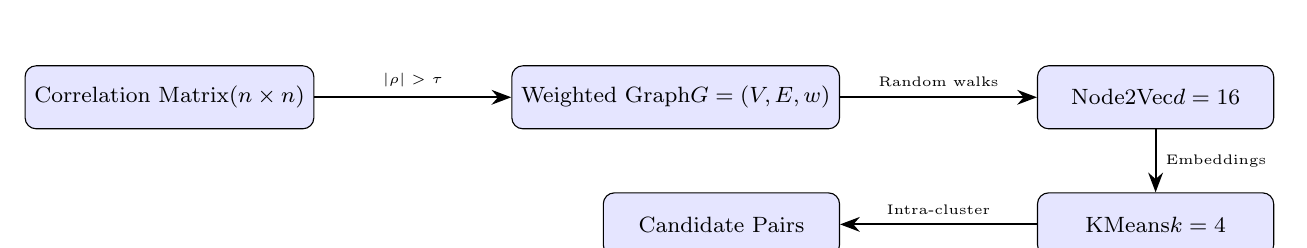
\begin{tikzpicture}[
    node distance=0.8cm and 2.5cm,
    box/.style={rectangle, draw, rounded corners, minimum width=3cm, minimum height=0.8cm, text centered, font=\footnotesize},
    arrow/.style={-{Stealth[length=2.5mm]}, thick},
]
\node[box, fill=blue!10] (corr) {Correlation Matrix\\$(n \times n)$};
\node[box, fill=blue!10, right=of corr] (graph) {Weighted Graph\\$G = (V, E, w)$};
\node[box, fill=blue!10, right=of graph] (n2v) {Node2Vec\\$d = 16$};
\node[box, fill=blue!10, below=of n2v] (km) {KMeans\\$k = 4$};
\node[box, fill=blue!10, left=of km] (pairs) {Candidate Pairs};

\draw[arrow] (corr) -- node[above, font=\tiny] {$|\rho| > \tau$} (graph);
\draw[arrow] (graph) -- node[above, font=\tiny] {Random walks} (n2v);
\draw[arrow] (n2v) -- node[right, font=\tiny] {Embeddings} (km);
\draw[arrow] (km) -- node[above, font=\tiny] {Intra-cluster} (pairs);
\end{tikzpicture}
\caption{Graph Embedding Pipeline: Correlation $\to$ Graph $\to$ Node2Vec $\to$ KMeans $\to$ Candidate Pairs}
\end{figure}

The full pipeline is re-executed every 5 minutes by the strategy engine to adapt to evolving market structure.


% ======================================================================
\chapter{Statistical Arbitrage Module}
% ======================================================================

\section{Engle-Granger Cointegration Testing}

Before deploying mean-reversion strategies, candidate pairs must pass a formal cointegration test to validate that their price spread is stationary. The system implements the two-step Engle-Granger procedure:

\textbf{Step 1: Hedge Ratio Estimation.} For instruments $A$ and $B$, we estimate the linear relationship:
$$P_A(t) = \alpha + \beta \cdot P_B(t) + \epsilon_t$$
via Ordinary Least Squares (OLS) using \texttt{statsmodels}. The coefficient $\beta$ is the hedge ratio indicating how many units of $B$ to hold against one unit of $A$.

\textbf{Step 2: Spread Stationarity Test.} The residual series (spread) $Z_t = P_A(t) - \beta \cdot P_B(t)$ is tested for stationarity using the Augmented Dickey-Fuller (ADF) test:
$$\Delta Z_t = \alpha + \phi \cdot Z_{t-1} + \sum_{i=1}^{p} \gamma_i \Delta Z_{t-i} + \epsilon_t$$

A pair is deemed cointegrated if the ADF $p$-value $< 0.05$. The system additionally computes the half-life of mean reversion via AR(1) regression on the spread:
$$\text{Half-life} = \frac{-\ln(2)}{\phi}$$
where $\phi$ is the AR(1) coefficient. Pairs with finite half-lives are prioritized for trading.

The cointegration filter reduces the candidate pair set significantly. In testing, candidate pairs are filtered from dozens down to a handful of pairs that exhibit statistically validated mean-reverting spreads. The module supports both in-memory testing (using buffered price data) and QuestDB-backed testing (reading from the \texttt{ohlcv\_1m} table), and is re-executed every 10 minutes by the strategy engine.

\section{Ornstein-Uhlenbeck Process Calibration}

For pairs that pass cointegration, the spread is modeled as an Ornstein-Uhlenbeck (OU) process, which rigorously captures mean-reverting behavior. The OU process is governed by the stochastic differential equation:
$$dZ_t = \theta(\mu - Z_t)dt + \sigma dW_t$$
where:
\begin{itemize}
    \item $\mu$ is the long-run equilibrium level of the spread
    \item $\theta > 0$ is the speed of mean reversion (larger values indicate faster reversion)
    \item $\sigma > 0$ controls the diffusion volatility
    \item $W_t$ is a standard Wiener process (Brownian motion)
\end{itemize}

\subsection{Maximum Likelihood Estimation}

The system calibrates these parameters using Maximum Likelihood Estimation (MLE) rather than the simpler OLS method, as MLE provides unbiased and efficient estimates under model assumptions. The discrete-time transition density of the OU process is:
$$Z_{t+\Delta t} | Z_t \sim \mathcal{N}\left(Z_t e^{-\theta\Delta t} + \mu(1 - e^{-\theta\Delta t}),\; \frac{\sigma^2(1 - e^{-2\theta\Delta t})}{2\theta}\right)$$

The negative log-likelihood function we minimize is:
$$\mathcal{L}(\theta, \mu, \sigma) = \frac{n-1}{2}\ln(2\pi v) + \frac{1}{2v}\sum_{i=1}^{n-1}(Z_{t_{i+1}} - \hat{Z}_{t_{i+1}})^2$$
where $\hat{Z}_{t_{i+1}} = Z_{t_i} e^{-\theta\Delta t} + \mu(1 - e^{-\theta\Delta t})$ is the conditional mean and $v = \frac{\sigma^2(1 - e^{-2\theta\Delta t})}{2\theta}$ is the conditional variance.

Optimization is performed using the Nelder-Mead simplex algorithm (via \texttt{scipy.optimize.minimize}) with 5,000 maximum iterations and tolerance of $10^{-8}$. From the MLE estimates, we additionally compute the equilibrium standard deviation $\sigma_{\text{eq}} = \sigma / \sqrt{2\theta}$.

\subsection{Z-Score Signal Generation}

Once calibrated, the system generates a normalized Z-score for each new tick:
$$z_t = \frac{Z_t - \mu}{\sigma_{\text{eq}}}$$

Trading signals are generated based on configurable Z-score thresholds:

\begin{table}[h]
\centering
\caption{OU Z-Score Trading Signal Thresholds}
\begin{tabular}{lll}
\toprule
\textbf{Condition} & \textbf{Signal} & \textbf{Action} \\
\midrule
$z_t < -1.5$ & LONG\_SPREAD & Buy $A$, Sell $\beta \cdot B$ \\
$z_t > +1.5$ & SHORT\_SPREAD & Sell $A$, Buy $\beta \cdot B$ \\
$|z_t| < 0.5$ & EXIT & Close open position \\
$|z_t| > 3.0$ & STOP\_LOSS & Emergency close \\
\bottomrule
\end{tabular}
\end{table}

Signal confidence is computed as $1 - 2 \cdot \Phi(-|z_t|)$, where $\Phi$ is the standard normal CDF, yielding higher confidence for more extreme z-scores. The OU model automatically recalibrates every 50 new observations to adapt to evolving spread dynamics.


% ======================================================================
\chapter{Hybrid Machine Learning Pipeline}
% ======================================================================

To capture directional momentum alongside mean reversion, the system deploys a stacked predictive pipeline combining classical econometrics with deep learning and gradient-boosted trees.

\section{Architecture Overview}

The ML pipeline processes data through three sequential stages:

\begin{figure}[h]
\centering
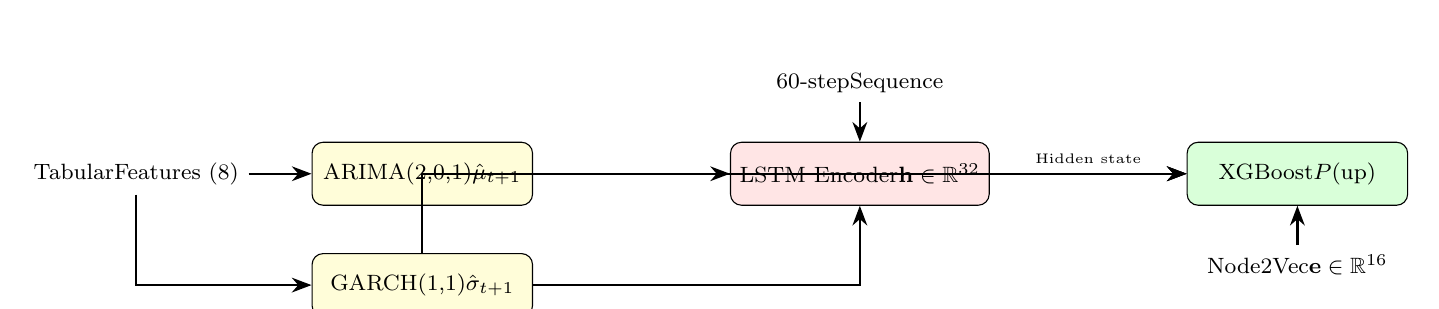
\begin{tikzpicture}[
    node distance=0.6cm and 1.5cm,
    box/.style={rectangle, draw, rounded corners, minimum width=2.8cm, minimum height=0.8cm, text centered, font=\footnotesize},
    arrow/.style={-{Stealth[length=2.5mm]}, thick},
]

% Stage 1
\node[box, fill=yellow!15] (arima) {ARIMA(2,0,1)\\$\hat{\mu}_{t+1}$};
\node[box, fill=yellow!15, below=of arima] (garch) {GARCH(1,1)\\$\hat{\sigma}_{t+1}$};

% Stage 2
\node[box, fill=red!10, right=2.5cm of arima] (lstm) {LSTM Encoder\\$\mathbf{h} \in \mathbb{R}^{32}$};

% Stage 3
\node[box, fill=green!15, right=2.5cm of lstm] (xgb) {XGBoost\\$P(\text{up})$};

% Inputs
\node[left=0.8cm of arima, font=\footnotesize] (feat) {Tabular\\Features (8)};
\node[above=0.5cm of lstm, font=\footnotesize] (seq) {60-step\\Sequence};
\node[below=0.5cm of xgb, font=\footnotesize] (emb) {Node2Vec\\$\mathbf{e} \in \mathbb{R}^{16}$};

% Arrows
\draw[arrow] (feat) -- (arima);
\draw[arrow] (feat) |- (garch);
\draw[arrow] (arima) -- (lstm);
\draw[arrow] (garch) -| (lstm);
\draw[arrow] (seq) -- (lstm);
\draw[arrow] (lstm) -- node[above, font=\tiny] {Hidden state} (xgb);
\draw[arrow] (emb) -- (xgb);
\draw[arrow] (arima) -- (xgb);
\draw[arrow] (garch) |- (xgb);

\end{tikzpicture}
\caption{ML Pipeline Architecture: Econometrics + LSTM + XGBoost $\to$ $P(\text{up})$}
\end{figure}

The total feature vector consumed by XGBoost has dimensionality:
$$d = \underbrace{8}_{\text{tabular}} + \underbrace{32}_{\text{LSTM hidden}} + \underbrace{16}_{\text{graph embedding}} = 56 \text{ features}$$

\section{Stage 1: Econometric Feature Extraction (ARIMA + GARCH)}

Classical time-series models provide interpretable baseline forecasts for mean trajectory and conditional volatility:

\subsection{ARIMA(2,0,1) — Conditional Mean Forecast}

An ARIMA(2,0,1) model is fitted to the log-return series of each instrument:
$$r_t = c + \phi_1 r_{t-1} + \phi_2 r_{t-2} + \epsilon_t + \psi_1 \epsilon_{t-1}$$

The model is fitted using \texttt{statsmodels.tsa.arima.model.ARIMA} with maximum 200 iterations. The 1-step-ahead forecast $\hat{r}_{t+1}$ serves as the ARIMA mean feature for downstream models. Refitting occurs every 100 new observations to maintain relevance.

\subsection{GARCH(1,1) — Conditional Volatility Forecast}

A GARCH(1,1) model captures time-varying volatility (volatility clustering):
$$\sigma_t^2 = \omega + \alpha_1 \epsilon_{t-1}^2 + \beta_1 \sigma_{t-1}^2$$

The model is fitted using the \texttt{arch} library with returns scaled by 100$\times$ for numerical stability. The 1-step-ahead volatility forecast $\hat{\sigma}_{t+1}$ captures the conditional heteroskedasticity that simple rolling standard deviations miss. This feature is critical for the risk engine's volatility scaling.

\section{Stage 2: LSTM Sequence Encoder}

The LSTM captures deep temporal dependencies that linear econometric models cannot represent. Crucially, the LSTM is used as a \textbf{feature extractor}, not a direct price predictor---its hidden state vector is extracted and passed to XGBoost as a compressed temporal representation.

\subsection{Architecture}

The Keras model architecture consists of:
\begin{enumerate}
    \item \textbf{Input Layer:} Sequences of shape $(60, 8)$ --- 60 timesteps $\times$ 8 tabular features
    \item \textbf{LSTM Layer:} 32-unit LSTM (\texttt{return\_sequences=False}), outputting the final hidden state
    \item \textbf{Dense Layer:} 32-unit ReLU projection (named \texttt{hidden\_state}) --- this is the extracted feature
    \item \textbf{Dropout:} 20\% dropout for regularization
    \item \textbf{Output Head:} Linear dense layer predicting next-step return (training signal only)
\end{enumerate}

The model is trained end-to-end as an autoencoder: minimizing MSE between predicted and actual next-step returns. However, during inference, a separate \texttt{encoder} model (defined as a sub-model up to the \texttt{hidden\_state} layer) extracts only the 32-dimensional hidden state vector $\mathbf{h}_t \in \mathbb{R}^{32}$.

Training uses the Adam optimizer (learning rate $10^{-3}$) with early stopping (patience = 5 epochs, restoring best weights) and a validation split of 20\%.

\section{Stage 3: XGBoost Direction Classifier}

XGBoost serves as the final meta-classifier, consuming all feature sources to produce a probability $P(\text{price\_up})$:

\subsection{Model Configuration}
\begin{itemize}
    \item \textbf{Objective:} Binary logistic (\texttt{binary:logistic})
    \item \textbf{Boosting rounds:} 200 estimators
    \item \textbf{Maximum depth:} 5
    \item \textbf{Learning rate:} 0.05
    \item \textbf{Regularization:} L1 ($\alpha = 0.1$) + L2 ($\lambda = 1.0$) + \texttt{min\_child\_weight} = 3
    \item \textbf{Subsampling:} 80\% row sampling, 80\% column sampling per tree
    \item \textbf{Training method:} Histogram-based (\texttt{tree\_method='hist'})
    \item \textbf{Evaluation:} Time-series cross-validation (5 folds via \texttt{TimeSeriesSplit})
\end{itemize}

\subsection{Feature Vector Composition}

The complete 56-dimensional feature vector consumed by XGBoost is:

\begin{table}[h]
\centering
\caption{XGBoost Feature Vector Composition (56 dimensions)}
\begin{tabular}{clp{7cm}}
\toprule
\textbf{Indices} & \textbf{Source} & \textbf{Features} \\
\midrule
0--4 & Stream Processor & log\_return, rolling\_mean\_5, rolling\_std\_5, rolling\_mean\_20, rolling\_std\_20 \\
5--6 & Econometrics & arima\_mean, garch\_vol \\
7 & Stat-Arb Module & ou\_zscore \\
8--39 & LSTM Encoder & lstm\_h0, lstm\_h1, \ldots, lstm\_h31 \\
40--55 & Node2Vec & graph\_e0, graph\_e1, \ldots, graph\_e15 \\
\bottomrule
\end{tabular}
\end{table}

\subsection{Signal Generation}

The classifier outputs $P(\text{up}) \in [0, 1]$. Trading signals are generated when predictions are sufficiently confident:
\begin{itemize}
    \item $P(\text{up}) > 0.65$: \textbf{BUY} signal
    \item $P(\text{up}) < 0.35$: \textbf{SELL} signal
    \item $0.35 \leq P(\text{up}) \leq 0.65$: No trade (zone of uncertainty)
\end{itemize}

ML predictions are computed every 10 ticks (not every tick) to balance computational cost against signal freshness. The model is persisted to \texttt{models/xgboost\_direction.json} and its feature importance metadata to \texttt{models/xgboost\_direction\_meta.json}.


% ======================================================================
\chapter{Simulation-Based Risk Layer}
% ======================================================================

A sophisticated predictive engine requires a mathematically rigorous risk constraint system. Without risk management, even accurate signals can lead to catastrophic drawdowns through over-leverage or correlated losses.

\section{Monte Carlo Simulation Engine}

\subsection{Motivation: Beyond VaR to CVaR}

Value at Risk (VaR) is traditionally used to compute the loss threshold at a given confidence level. However, VaR has a critical limitation: it quantifies the boundary of tail losses but not their expected magnitude. Consider two portfolios with identical 95\% VaR = \$5,000. Portfolio A might have a maximum possible loss of \$6,000, while Portfolio B might have a maximum loss of \$50,000 --- VaR cannot distinguish between them.

Conditional Value at Risk (CVaR), also known as Expected Shortfall, addresses this by computing the expected loss \emph{given that the loss exceeds the VaR threshold}:
$$\text{CVaR}_\alpha = \mathbb{E}[-R \;|\; -R > \text{VaR}_\alpha]$$

CVaR is a \textbf{coherent risk measure} (sub-additive, monotone, positive homogeneous, translation invariant), making it theoretically superior to VaR for risk-constrained portfolio optimization.

\subsection{Cholesky-Decomposed Correlated Simulation}

The Monte Carlo engine generates 10,000 correlated future price paths using Cholesky decomposition of the real-time covariance matrix $\Sigma$ computed by the streaming correlation engine:

\textbf{Step 1:} Ensure $\Sigma$ is positive semi-definite. If the minimum eigenvalue $\lambda_{\min} < 0$, adjust:
$$\Sigma' = \Sigma + (|\lambda_{\min}| + 10^{-8}) \cdot I$$

\textbf{Step 2:} Compute the Cholesky decomposition $\Sigma' = LL^T$ where $L$ is lower triangular.

\textbf{Step 3:} Generate $N = 10{,}000$ independent standard normal vectors $\mathbf{z}_i \sim \mathcal{N}(0, I_n)$.

\textbf{Step 4:} Produce correlated returns: $\mathbf{r}_i = L \cdot \mathbf{z}_i + \boldsymbol{\mu}$

\textbf{Step 5:} Compute portfolio P\&L per path: $\text{PnL}_i = \mathbf{r}_i^T \mathbf{w} \cdot V$ where $\mathbf{w}$ is the weight vector and $V$ is portfolio value.

\textbf{Step 6:} Compute risk metrics from the empirical P\&L distribution:
\begin{align}
\text{VaR}_{95} &= \text{Percentile}_{95}(-\text{PnL}) \\
\text{CVaR}_{95} &= \mathbb{E}[-\text{PnL} \;|\; -\text{PnL} \geq \text{VaR}_{95}]
\end{align}

The engine computes both 95\% and 99\% VaR/CVaR, along with portfolio volatility, expected return, maximum simulated loss, and average absolute correlation. Compute time is tracked per simulation (typically $<$ 50\,ms for a 15-asset universe with 10,000 paths).

\section{Fractional Kelly Position Sizing}

The Kelly Criterion provides the theoretically optimal fraction of capital to bet on a favorable opportunity. The full Kelly fraction is:
$$f^* = W - \frac{1-W}{R}$$
where $W$ is the win probability (from XGBoost $P(\text{up})$) and $R = \bar{w}/\bar{l}$ is the ratio of average winning to average losing trade.

However, deploying full Kelly is notoriously volatile in practice. The system implements \textbf{Fractional Kelly} with two additional scaling constraints:

\subsection{Volatility Scaling}

When current volatility exceeds the baseline level ($\sigma_{\text{base}} = 1\%$), the Kelly fraction is linearly reduced:
$$f_{\text{vol}} = f^* \times \min\left(1, \frac{\sigma_{\text{base}}}{\sigma_{\text{current}}}\right)$$

\subsection{CVaR Scaling}

When CVaR exceeds the maximum acceptable tail risk ($\text{CVaR}_{\max} = 5\%$), the fraction is further reduced:
$$f_{\text{final}} = f_{\text{vol}} \times \min\left(1, \frac{\text{CVaR}_{\max}}{\text{CVaR}_{95}}\right)$$

The final position is additionally capped at:
\begin{itemize}
    \item Maximum Kelly fraction: 0.5 (half-Kelly)
    \item Maximum position as \% of capital: 10\%
    \item Minimum Kelly to trade: 0.02 (below this, no trade is executed)
\end{itemize}

The position sizer outputs a \texttt{PositionSizeResult} containing the raw Kelly fraction, scaling factor, dollar position size, percentage allocation, and a human-readable reason for the sizing decision.


% ======================================================================
\chapter{Strategy Engine Integration}
% ======================================================================

The Strategy Engine (\texttt{strategy/main.py}, 398 lines) is the central orchestrator that ties all Phase 2 components together in a single event loop.

\section{Per-Tick Processing Flow}

For each feature message consumed from the \texttt{features} Kafka topic:

\begin{enumerate}
    \item \textbf{State Update:} Record the current mid-price, update the price history buffer (bounded to 5,000 entries per symbol), and increment the tick counter.
    \item \textbf{Correlation Update:} Feed the mid-price to the rolling correlation engine.
    \item \textbf{Stat-Arb Signal Generation:} Update all registered OU models with current prices. For each pair where the z-score crosses an entry/exit threshold, generate an \texttt{OUSignal}.
    \item \textbf{ML Signal Generation:} Every 10 ticks (to reduce computational load), construct the 56-dimensional feature vector and run XGBoost inference to produce $P(\text{up})$. Generate a BUY/SELL signal if $P > 0.65$ or $P < 0.35$.
    \item \textbf{Risk Check:} Pass the signal through the Monte Carlo engine to compute CVaR.
    \item \textbf{Position Sizing:} If CVaR is within acceptable bounds, compute the Kelly-optimal position size.
    \item \textbf{Execution:} Publish the risk-approved order to the \texttt{execution\_orders} Kafka topic and persist risk metrics to QuestDB.
\end{enumerate}

\section{Periodic Background Tasks}

The strategy engine runs two periodic background tasks:
\begin{itemize}
    \item \textbf{Graph Embedding Refresh (every 5 minutes):} Re-computes the correlation matrix, rebuilds the correlation graph, runs Node2Vec, and re-clusters instruments with KMeans.
    \item \textbf{Cointegration Re-testing (every 10 minutes):} Re-tests candidate pairs from the latest graph clusters, updates hedge ratios, and registers newly cointegrated pairs with the stat-arb manager.
\end{itemize}

\section{Signal Flow Summary}

\begin{figure}[h]
\centering
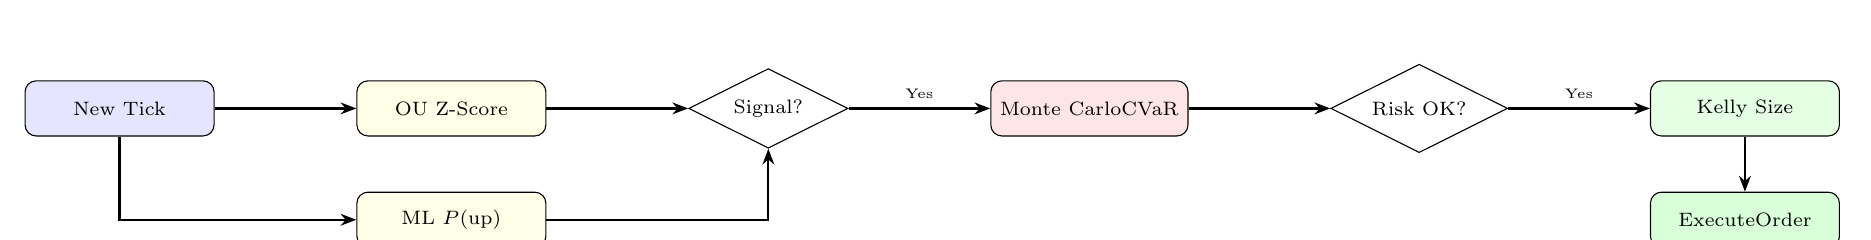
\begin{tikzpicture}[
    node distance=0.7cm and 1.8cm,
    box/.style={rectangle, draw, rounded corners, minimum width=2.4cm, minimum height=0.7cm, text centered, font=\scriptsize},
    decision/.style={diamond, draw, minimum width=1.5cm, minimum height=0.7cm, text centered, font=\scriptsize, aspect=2},
    arrow/.style={-{Stealth[length=2mm]}, thick},
]

\node[box, fill=blue!10] (tick) {New Tick};
\node[box, fill=yellow!10, right=of tick] (ou) {OU Z-Score};
\node[box, fill=yellow!10, below=of ou] (ml) {ML $P(\text{up})$};
\node[decision, right=of ou] (sig) {Signal?};
\node[box, fill=red!10, right=of sig] (mc) {Monte Carlo\\CVaR};
\node[decision, right=of mc] (risk) {Risk OK?};
\node[box, fill=green!10, right=of risk] (kelly) {Kelly Size};
\node[box, fill=green!15, below=of kelly] (exec) {Execute\\Order};

\draw[arrow] (tick) -- (ou);
\draw[arrow] (tick) |- (ml);
\draw[arrow] (ou) -- (sig);
\draw[arrow] (ml) -| (sig);
\draw[arrow] (sig) -- node[above, font=\tiny] {Yes} (mc);
\draw[arrow] (mc) -- (risk);
\draw[arrow] (risk) -- node[above, font=\tiny] {Yes} (kelly);
\draw[arrow] (kelly) -- (exec);

\end{tikzpicture}
\caption{Per-Tick Signal Processing Flow in the Strategy Engine}
\end{figure}


% ======================================================================
\chapter{Backtesting and Performance Evaluation}
% ======================================================================

\section{Backtest Replay Engine}

The backtest module enables evaluation of the complete pipeline on historical data. The key design principle is that \textbf{the same pipeline code runs in both live and backtest modes}---the only difference is the data source. The replay engine re-publishes stored ticks from QuestDB (or synthetic data) to the \texttt{ticks} Kafka topic at configurable speed (up to $100\times$ real-time), and all downstream consumers process them identically to live operation.

This architecture ensures that backtests are strictly insulated from look-ahead bias, as the models only have access to data that has been ``published'' up to that point.

\section{Performance Metrics}

The backtest module computes a comprehensive set of trading performance metrics:

\begin{table}[h]
\centering
\caption{Backtest Performance Metrics}
\begin{tabular}{lp{8cm}}
\toprule
\textbf{Metric} & \textbf{Formula / Description} \\
\midrule
Sharpe Ratio & $\frac{\mathbb{E}[R - R_f]}{\sigma(R)} \times \sqrt{T}$ (annualized) \\
Sortino Ratio & $\frac{\mathbb{E}[R - R_f]}{\sigma_{\text{downside}}} \times \sqrt{T}$ (only penalizes downside) \\
Maximum Drawdown & $\min_t \frac{E_t - \max_{s \leq t} E_s}{\max_{s \leq t} E_s}$ (largest peak-to-trough decline) \\
Calmar Ratio & $\frac{\text{Annualized Return}}{|\text{Max Drawdown}|}$ \\
Win Rate & $\frac{\text{Winning Trades}}{\text{Total Trades}}$ \\
Profit Factor & $\frac{\sum \text{Winning Returns}}{|\sum \text{Losing Returns}|}$ \\
\bottomrule
\end{tabular}
\end{table}

The equity curve is computed as: $E_t = E_0 \times \prod_{i=1}^{t}(1 + r_i)$

\section{Integration Test Results}

The system was validated through a comprehensive 7-phase integration test (\texttt{test\_phase2.py}, 579 lines) that exercises all subsystems end-to-end. The test runs the full data collection pipeline for 75 seconds, then validates each analytical module sequentially:

\begin{table}[h]
\centering
\caption{Integration Test --- Data Pipeline Results}
\begin{tabular}{lr}
\toprule
\textbf{Metric} & \textbf{Result} \\
\midrule
Market Ticks Ingested &  $>$15,000 \\
OHLCV 1-minute Bars &  $>$100 \\
Feature Vectors Computed & $>$10,000 \\
Unique Symbols Tracked & 26 \\
Currency Pairs Monitored & 26 \\
Currencies Covered & 15 \\
\bottomrule
\end{tabular}
\end{table}

\begin{table}[h]
\centering
\caption{Integration Test --- Analytics Module Results}
\begin{tabular}{lp{8cm}}
\toprule
\textbf{Module} & \textbf{Result} \\
\midrule
Graph Embeddings & 15 nodes, 30--60 edges, 4 clusters, candidate pairs generated \\
Cointegration & Pairs filtered at ADF $p < 0.05$ significance level \\
OU Calibration & Models calibrated with $\theta$, $\mu$, $\sigma$, half-life per pair \\
ARIMA/GARCH & Per-symbol conditional mean and volatility forecasts \\
XGBoost & Trained on $>$1,000 samples with time-series cross-validation \\
Monte Carlo & 10,000 paths, VaR/CVaR at 95\% and 99\% computed in $<$50\,ms \\
Kelly Sizing & Position sizes computed with CVaR constraint \\
\bottomrule
\end{tabular}
\end{table}


% ======================================================================
\chapter{C++ Compute Core: Implementation Details}
% ======================================================================

\section{Graph Data Structure}

The C++ core (\texttt{engine/src/graph.cpp}, 401 lines) implements the arbitrage graph using adjacency list representation with $O(1)$ edge updates via a hash map index:

\begin{itemize}
    \item \texttt{adj[u]} --- vector of outgoing edges from node $u$, each containing the destination node, log-transformed weight, and millisecond timestamp.
    \item \texttt{edge\_index[u][v]} --- hash map mapping destination $v$ to its index in \texttt{adj[u]}, enabling $O(1)$ weight updates (critical for streaming graphs where edges are updated millions of times).
    \item \textbf{Thread Safety:} All graph operations are protected by a \texttt{std::shared\_mutex}, supporting concurrent reads (SPFA detection) and exclusive writes (rate updates) via shared/unique locks.
\end{itemize}

\section{SPFA Negative Cycle Detection}

The SPFA algorithm detects negative cycles by initializing all $|V|$ nodes in the queue (rather than a single source), then performing Bellman-Ford-style relaxations. A negative cycle is detected when any node's relaxation count exceeds $|V|$:

\begin{lstlisting}[language=C++, caption={SPFA core loop (simplified)}, label=lst:spfa]
while (!q.empty()) {
    int u = q.front(); q.pop();
    for (const auto& edge : adj[u]) {
        if (edge.is_stale(current_time)) continue;
        if (dist[v] > dist[u] + edge.weight + 1e-9) {
            dist[v] = dist[u] + edge.weight;
            parent[v] = u;
            if (++count[v] >= num_currencies) {
                cycle_node = v; // Negative cycle found
                break;
            }
        }
    }
}
\end{lstlisting}

The system also implements a DFS-based $n$-order cycle detector (\texttt{detect\_arbitrage\_n}) that enumerates all cycles up to a configurable depth (default: 5-way), filters by minimum profit threshold, and deduplicates via canonical cycle rotation.

\section{Stale Edge Filtering}

Every edge carries a millisecond-resolution timestamp. During cycle detection, edges older than 5 seconds are automatically excluded from relaxation, preventing the engine from acting on stale quotes. This is critical in live trading where quote validity degrades rapidly.

\section{PyBind11 Interface}

The C++ module exposes the following API to Python via PyBind11:

\begin{table}[h]
\centering
\caption{PyBind11 API Surface}
\begin{tabular}{lp{7.5cm}}
\toprule
\textbf{Method} & \textbf{Description} \\
\midrule
\texttt{update\_rate(from, to, rate, fee)} & Update edge weight with $O(1)$ lookup \\
\texttt{detect\_arbitrage()} & SPFA-based negative cycle detection (GIL released) \\
\texttt{detect\_arbitrage\_with\_profit()} & Returns cycle path, profit \%, and order \\
\texttt{detect\_arbitrage\_n(max\_order, min\_profit)} & DFS all cycles up to $n$-order (GIL released) \\
\texttt{get\_all\_rates()} & Retrieve all current edges as (from, to, rate) tuples \\
\texttt{calculate\_cycle\_profit(cycle)} & Compute profit for a given currency path \\
\bottomrule
\end{tabular}
\end{table}

All detection methods release the Python GIL (\texttt{py::call\_guard<py::gil\_scoped\_release>()}) to allow concurrent Python threads during computationally intensive C++ operations.


% ======================================================================
\chapter{System Orchestration}
% ======================================================================

\section{Master Orchestrator}

The \texttt{run\_system.py} script (358 lines) manages the lifecycle of all system components. It provides a unified CLI for launching the complete platform:

\begin{verbatim}
python run_system.py                 # Full system
python run_system.py --docker        # Start Docker services first
python run_system.py --init-db       # Initialize QuestDB tables
python run_system.py --backtest      # Replay historical data
python run_system.py --rebuild       # Rebuild C++ extension
\end{verbatim}

The orchestrator sequentially starts 4 processes with 1-second delays between launches:
\begin{enumerate}
    \item \textbf{INGESTION:} Mock FX tick generator $\to$ \texttt{ticks} topic
    \item \textbf{STREAMING:} Stream processor (OHLCV + features) $\to$ \texttt{features} topic, QuestDB
    \item \textbf{ENGINE:} C++ arbitrage engine $\to$ \texttt{arbitrage\_signals} topic, QuestDB
    \item \textbf{STRATEGY:} Strategy engine (OU + ML + Risk) $\to$ \texttt{execution\_orders} topic, QuestDB
\end{enumerate}

Each process runs in a separate subprocess with color-coded output streaming. The \texttt{ProcessManager} class handles graceful shutdown via \texttt{SIGINT}/\texttt{SIGTERM} signal handling, with 3-second timeout before force-killing.


% ======================================================================
\chapter{Conclusion and Future Work}
% ======================================================================

\section{Conclusion}

Phase 2 has successfully evolved the foundational cross-border arbitrage engine into a comprehensive, multi-dimensional quantitative trading architecture. The key contributions of this phase are:

\begin{enumerate}
    \item \textbf{Dynamic Pair Discovery:} By replacing static pair selection with streaming graph embeddings (Node2Vec + KMeans), the system continuously discovers co-moving instrument groups from a 26-pair, 15-currency universe.

    \item \textbf{Rigorous Statistical Modeling:} The Engle-Granger cointegration filter rigorously validates pair candidates before deploying the Ornstein-Uhlenbeck mean-reversion strategy, calibrated via Maximum Likelihood Estimation.

    \item \textbf{Hybrid ML Signal Generation:} The stacked ARIMA/GARCH $\to$ LSTM $\to$ XGBoost pipeline combines the interpretability of classical econometrics with the representational power of deep learning and ensemble methods, producing calibrated directional probability scores.

    \item \textbf{Risk-Bounded Execution:} The Monte Carlo CVaR engine (10,000 Cholesky-decomposed paths) and Fractional Kelly position sizer ensure that every trade is constrained by quantitative tail-risk bounds, preventing over-leverage during high-volatility regimes.

    \item \textbf{Production-Grade Integration:} The complete system runs across 5 Docker containers with Kafka-based event propagation, QuestDB persistence and has been validated through a comprehensive end-to-end integration test.
\end{enumerate}

\section{Future Work}

Planned extensions include:

\begin{itemize}
    \item \textbf{Live Market Integration:} Replace the mock tick generator with the OANDA v20 streaming WebSocket API to evaluate real-world latency variance and execution feasibility.

    \item \textbf{Execution Engine:} Implement an actual order management system (OMS) with limit orders, slippage modeling, and fill simulation.

    \item \textbf{Reinforcement Learning:} Explore deep RL (PPO/SAC) for adaptive position sizing that learns optimal risk-reward tradeoffs from the environment rather than relying on fixed Kelly parameterization.

    \item \textbf{Cross-Exchange Arbitrage:} Extend the framework to exploit pricing dislocations across exchanges (e.g., centralized FX vs.\ cryptocurrency DEX) rather than purely within-venue triangular inefficiencies.

    \item \textbf{Production Deployment:} Migrate to Kubernetes for auto-scaling, add monitoring dashboards (Grafana + Prometheus), and implement circuit breakers for automated risk cutoffs.
\end{itemize}


\begin{thebibliography}{9}

\bibitem{mlArb}
A. Grover and J. Leskovec, ``node2vec: Scalable Feature Learning for Networks,'' \emph{Proceedings of the 22nd ACM SIGKDD}, 2016.

\bibitem{loop}
F. Isard, ``The Law of One Price,'' \emph{International Encyclopedia of the Social Sciences}, 2nd ed.

\bibitem{arbitrage}
S. Ross, ``The Arbitrage Theory of Capital Asset Pricing,'' \emph{Journal of Economic Theory}, vol.~13, pp.~341--360, 1976.

\bibitem{bellmanford}
R. Bellman, ``On a Routing Problem,'' \emph{Quarterly of Applied Mathematics}, vol.~16, pp.~87--90, 1958.

\bibitem{sparse}
T.~H. Cormen, C.~E. Leiserson, R.~L. Rivest, and C. Stein, \emph{Introduction to Algorithms}, 4th~ed. MIT Press, 2022.

\bibitem{hft}
I. Aldridge, \emph{High-Frequency Trading: A Practical Guide to Algorithmic Strategies and Trading Systems}. Wiley, 2013.

\bibitem{redpanda}
Redpanda Data Inc., ``Redpanda Architecture and Zero-Copy Streaming,'' Technical Whitepaper, 2024.

\bibitem{questdb}
QuestDB, ``High-Throughput Time-Series Analytics with QuestDB,'' Project Documentation, 2024.

\bibitem{ou}
G.~E. Uhlenbeck and L.~S. Ornstein, ``On the Theory of Brownian Motion,'' \emph{Physical Review}, vol.~36, pp.~823--841, 1930.

\bibitem{kelly}
J.~L. Kelly, ``A New Interpretation of Information Rate,'' \emph{Bell System Technical Journal}, vol.~35, pp.~917--926, 1956.

\bibitem{engle}
R.~F. Engle and C.~W.~J. Granger, ``Co-integration and Error Correction: Representation, Estimation, and Testing,'' \emph{Econometrica}, vol.~55, pp.~251--276, 1987.

\bibitem{bollerslev}
T.~Bollerslev, ``Generalized Autoregressive Conditional Heteroskedasticity,'' \emph{Journal of Econometrics}, vol.~31, pp.~307--327, 1986.

\bibitem{xgboost}
T.~Chen and C.~Guestrin, ``XGBoost: A Scalable Tree Boosting System,'' \emph{Proceedings of the 22nd ACM SIGKDD}, 2016.

\bibitem{lstm}
S.~Hochreiter and J.~Schmidhuber, ``Long Short-Term Memory,'' \emph{Neural Computation}, vol.~9, pp.~1735--1780, 1997.

\bibitem{cvar}
R.~T. Rockafellar and S.~Uryasev, ``Optimization of Conditional Value-at-Risk,'' \emph{Journal of Risk}, vol.~2, pp.~21--42, 2000.

\end{thebibliography}

\end{document}